% Practice Test 13 — Virginia Edition
% Questions: 30 (18 MC + 12 SA)
% Generated by scripts/generate_practice_tests.py

\begin{practiceQuestion}{1-4-q16}{mc}
\begin{questionText}
A printer prints $18$ pages per minute. How long will it take to print $270$ pages? Use the equation $p = 18m$.
\end{questionText}
\choiceA{$10$ minutes}
\choiceB{$15$ minutes}
\choiceC{$18$ minutes}
\choiceD{$20$ minutes}
\correctAnswer{B}
\explanation{$270 = 18m$, so $m = 270 \div 18 = 15$ minutes.}
\end{practiceQuestion}

\begin{practiceQuestion}{2-1-q18}{mc}
\begin{questionText}
Mia scored $85\%$ on a test with $60$ questions. How many questions did she answer correctly?
\end{questionText}
\choiceA{$48$}
\choiceB{$50$}
\choiceC{$51$}
\choiceD{$54$}
\correctAnswer{C}
\explanation{$85\% = 0.85$. Multiply: $0.85 \times 60 = 51$ questions correct.}
\end{practiceQuestion}

\begin{practiceQuestion}{2-2-q14}{mc}
\begin{questionText}
$27$ out of $180$ students earned an A on the exam. What percent earned an A?
\end{questionText}
\choiceA{$12\%$}
\choiceB{$15\%$}
\choiceC{$18\%$}
\choiceD{$27\%$}
\correctAnswer{B}
\explanation{$\frac{27}{180} = \frac{p}{100}$. Cross-multiply: $180p = 2700$. Divide: $p = 15\%$.}
\end{practiceQuestion}

\begin{practiceQuestion}{2-3-q19}{sa}
\begin{questionText}
A puppy weighed $6$ pounds and now weighs $9$ pounds. What is the percent increase in weight?


\numberLine[1]{6}{10}
\end{questionText}
\correctAnswer{$50\%$}
\explanation{Change: $9 - 6 = 3$. Percent increase: $3 \div 6 = 0.50 = 50\%$.}
\end{practiceQuestion}

\begin{practiceQuestion}{2-7-q30}{gsa}
\begin{questionText}
The bar graph shows the estimated and actual amounts of water (in liters) collected during an experiment over three days. On which day was the percent error the largest, and what was it?

\begin{center}
\begin{tikzpicture}[scale=0.5]
  \draw[thick,->] (0,0) -- (0,6.5) node[above]{\small Liters};
  \draw[thick,->] (0,0) -- (10.5,0);
  % Day 1: est 10, actual 8
  \fill[funBlue!60] (0.5,0) rectangle (1.5,5);
  \fill[funGreen!60] (1.5,0) rectangle (2.5,4);
  % Day 2: est 6, actual 5
  \fill[funBlue!60] (3.5,0) rectangle (4.5,3);
  \fill[funGreen!60] (4.5,0) rectangle (5.5,2.5);
  % Day 3: est 8, actual 10
  \fill[funBlue!60] (6.5,0) rectangle (7.5,4);
  \fill[funGreen!60] (7.5,0) rectangle (8.5,5);
  \node[below,font=\small] at (1.5,0) {Day 1};
  \node[below,font=\small] at (4.5,0) {Day 2};
  \node[below,font=\small] at (7.5,0) {Day 3};
  \foreach \y/\lab in {1/2,2/4,3/6,4/8,5/10,6/12} {
    \draw (-0.1,\y) -- (0.1,\y) node[left,font=\small,xshift=-2pt] {\lab};
  }
  \node[above,font=\scriptsize,funBlue] at (1,5) {$10$};
  \node[above,font=\scriptsize,funGreen!80!black] at (2,4) {$8$};
  \node[above,font=\scriptsize,funBlue] at (4,3) {$6$};
  \node[above,font=\scriptsize,funGreen!80!black] at (5,2.5) {$5$};
  \node[above,font=\scriptsize,funBlue] at (7,4) {$8$};
  \node[above,font=\scriptsize,funGreen!80!black] at (8,5) {$10$};
  % Legend
  \fill[funBlue!60] (0.5,6.3) rectangle (1,6.7);
  \node[right,font=\scriptsize] at (1.1,6.5) {Estimated};
  \fill[funGreen!60] (3.5,6.3) rectangle (4,6.7);
  \node[right,font=\scriptsize] at (4.1,6.5) {Actual};
\end{tikzpicture}
\end{center}
\end{questionText}
\correctAnswer{Day 1 with $25\%$ error}
\explanation{Day 1: $|10-8|/8 = 25\%$. Day 2: $|6-5|/5 = 20\%$. Day 3: $|8-10|/10 = 20\%$. Day 1 has the largest percent error at $25\%$.}
\end{practiceQuestion}

\begin{practiceQuestion}{3-2-q22}{sa}
\begin{questionText}
What is $(-18) + 18$?
\end{questionText}
\correctAnswer{$0$}
\explanation{$-18$ and $18$ are additive inverses (opposites). Their sum is always $0$.}
\end{practiceQuestion}

\begin{practiceQuestion}{3-3-q01}{mc}
\begin{questionText}
What is $10 - 16$?
\end{questionText}
\choiceA{$6$}
\choiceB{$-6$}
\choiceC{$26$}
\choiceD{$-26$}
\correctAnswer{B}
\explanation{Rewrite as $10 + (-16) = -6$. The larger absolute value ($16$) is negative.}
\end{practiceQuestion}

\begin{practiceQuestion}{3-4-q15}{mc}
\begin{questionText}
Which expression has the smallest (most negative) value?
\end{questionText}
\choiceA{$-0.5 + 0.3$}
\choiceB{$-0.8 - 0.4$}
\choiceC{$0.6 + (-0.9)$}
\choiceD{$-0.1 - 0.2$}
\correctAnswer{B}
\explanation{A: $-0.2$. B: $-1.2$. C: $-0.3$. D: $-0.3$. The most negative is $-1.2$.}
\end{practiceQuestion}

\begin{practiceQuestion}{4-3-q21}{sa}
\begin{questionText}
Expand $\frac{3}{4}(8a - 12)$.


\fractionCircle{3}{4}
\end{questionText}
\correctAnswer{$6a - 9$}
\explanation{$\frac{3}{4} \times 8a = 6a$ and $\frac{3}{4} \times (-12) = -9$. Result: $6a - 9$.}
\end{practiceQuestion}

\begin{practiceQuestion}{4-4-q26}{gmc}
\begin{questionText}
The area model below represents a factored expression. Which factored form matches the model?

\begin{center}
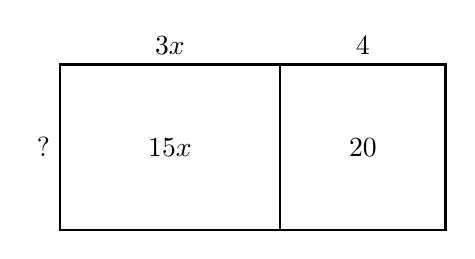
\begin{tikzpicture}[scale=0.7]
  \draw[thick] (0,0) rectangle (7,3);
  \draw[thick] (4,0) -- (4,3);
  \node[left] at (0,1.5) {?};
  \node[above] at (2,3) {$3x$};
  \node[above] at (5.5,3) {$4$};
  \node at (2,1.5) {$15x$};
  \node at (5.5,1.5) {$20$};
\end{tikzpicture}
\end{center}
\end{questionText}
\choiceA{$5(3x + 4)$}
\choiceB{$3(5x + 4)$}
\choiceC{$4(3x + 5)$}
\choiceD{$15(x + 20)$}
\correctAnswer{A}
\explanation{The width must satisfy: $? \times 3x = 15x$ and $? \times 4 = 20$. So $? = 5$. The factored form is $5(3x + 4) = 15x + 20$.}
\end{practiceQuestion}

\begin{practiceQuestion}{5-4-q06}{mc}
\begin{questionText}
Solve $-0.4y + 2 = 6$.
\end{questionText}
\choiceA{$y = 10$}
\choiceB{$y = -10$}
\choiceC{$y = 20$}
\choiceD{$y = -20$}
\correctAnswer{B}
\explanation{Subtract $2$: $-0.4y = 4$. Divide by $-0.4$: $y = -10$. Check: $-0.4(-10) + 2 = 4 + 2 = 6$ \checkmark.}
\end{practiceQuestion}

\begin{practiceQuestion}{5-5-q20}{sa}
\begin{questionText}
Solve $-5n + 10 \leq -15$.
\end{questionText}
\correctAnswer{$n \geq 5$}
\explanation{Subtract $10$: $-5n \leq -25$. Divide by $-5$ and flip: $n \geq 5$.}
\end{practiceQuestion}

\begin{practiceQuestion}{5-6-q16}{mc}
\begin{questionText}
Solve $\dfrac{x}{2} - 3 > 1$ and describe the graph.
\end{questionText}
\choiceA{Open circle at $8$, shade right}
\choiceB{Closed circle at $8$, shade right}
\choiceC{Open circle at $4$, shade right}
\choiceD{Open circle at $8$, shade left}
\correctAnswer{A}
\explanation{Add $3$: $\frac{x}{2} > 4$. Multiply by $2$: $x > 8$. Open circle at $8$, shade right.}
\end{practiceQuestion}

\begin{practiceQuestion}{6-1-q08}{mc}
\begin{questionText}
A scale drawing of a building uses $1$ in $= 10$ ft. The building is $85$ ft tall. How tall is it on the drawing?
\end{questionText}
\choiceA{$8$ in}
\choiceB{$8.5$ in}
\choiceC{$85$ in}
\choiceD{$850$ in}
\correctAnswer{B}
\explanation{Divide actual length by the scale factor: $85 \div 10 = 8.5$ in.}
\end{practiceQuestion}

\begin{practiceQuestion}{6-2-q23}{sa}
\begin{questionText}
A park is drawn at scale $1$ cm $= 50$ m. The park is $8$ cm wide on this drawing. If the new drawing must show the park as $4$ cm wide, what scale should the new drawing use?
\end{questionText}
\correctAnswer{$1$ cm $= 100$ m}
\explanation{Actual width: $8 \times 50 = 400$ m. New scale: $400 \div 4 = 100$ m per cm.}
\end{practiceQuestion}

\begin{practiceQuestion}{6-5-q12}{mc}
\begin{questionText}
A rectangular prism is sliced with a diagonal cut from one edge of the top to the opposite edge of the bottom. What is a possible cross-section?
\end{questionText}
\choiceA{Circle}
\choiceB{Triangle}
\choiceC{Hexagon}
\choiceD{Rectangle}
\correctAnswer{D}
\explanation{A diagonal slice through a rectangular prism from edge to edge can produce a rectangle (or a parallelogram, depending on the angle). A diagonal from top edge to opposite bottom edge typically gives a rectangle.}
\end{practiceQuestion}

\begin{practiceQuestion}{6-6-q09}{mc}
\begin{questionText}
An angle is $4$ times its supplement. What is the angle?
\end{questionText}
\choiceA{$36°$}
\choiceB{$45°$}
\choiceC{$120°$}
\choiceD{$144°$}
\correctAnswer{D}
\explanation{Let the supplement be $x$. The angle is $4x$. Sum: $x + 4x = 180$. So $5x = 180$ and $x = 36°$. The angle: $4(36) = 144°$.}
\end{practiceQuestion}

\begin{practiceQuestion}{6-7-q14}{mc}
\begin{questionText}
A rectangle has vertices $A(1, 1)$, $B(5, 1)$, $C(5, 3)$, $D(1, 3)$. It is translated left $3$ and up $4$. What are the coordinates of $C'$?
\end{questionText}
\choiceA{$(2, 7)$}
\choiceB{$(8, 7)$}
\choiceC{$(2, -1)$}
\choiceD{$(8, -1)$}
\correctAnswer{A}
\explanation{$C(5, 3)$: left $3$ means $5 - 3 = 2$, up $4$ means $3 + 4 = 7$. So $C'(2, 7)$.}
\end{practiceQuestion}

\begin{practiceQuestion}{6-8-q27}{gmc}
\begin{questionText}
The diagram shows two similar triangles. Find the missing side length $n$.

\begin{center}
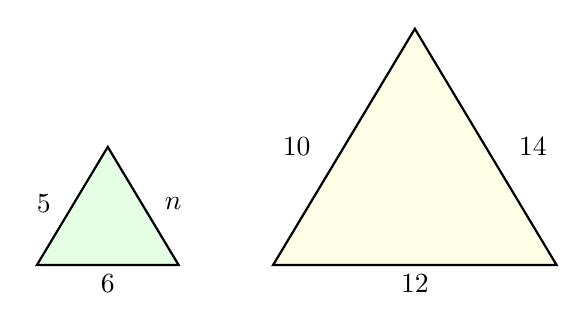
\begin{tikzpicture}[scale=0.6]
  % Small triangle
  \draw[thick,fill=green!10] (0,0) -- (3,0) -- (1.5,2.5) -- cycle;
  \node[below] at (1.5,0) {$6$};
  \node[left] at (0.5,1.3) {$5$};
  \node[right] at (2.5,1.3) {$n$};
  % Large triangle
  \draw[thick,fill=yellow!10] (5,0) -- (11,0) -- (8,5) -- cycle;
  \node[below] at (8,0) {$12$};
  \node[left] at (6,2.5) {$10$};
  \node[right] at (10,2.5) {$14$};
\end{tikzpicture}
\end{center}
\end{questionText}
\choiceA{$4$}
\choiceB{$7$}
\choiceC{$8$}
\choiceD{$9$}
\correctAnswer{B}
\explanation{Scale factor: $\frac{6}{12} = 0.5$ (or $\frac{5}{10} = 0.5$). $n = 14 \times 0.5 = 7$.}
\end{practiceQuestion}

\begin{practiceQuestion}{7-4-q08}{mc}
\begin{questionText}
A composite shape is made of a rectangle $7$ m by $4$ m with a semicircle of diameter $4$ m on one short side. What is the total area? Use $\pi \approx 3.14$.
\end{questionText}
\choiceA{$28$ m$^2$}
\choiceB{$34.28$ m$^2$}
\choiceC{$40.56$ m$^2$}
\choiceD{$53.12$ m$^2$}
\correctAnswer{B}
\explanation{Rectangle: $7 \times 4 = 28$ m$^2$. Semicircle: $\frac{1}{2} \times 3.14 \times 2^2 = \frac{1}{2} \times 3.14 \times 4 = 6.28$ m$^2$. Total: $28 + 6.28 = 34.28$ m$^2$.}
\end{practiceQuestion}

\begin{practiceQuestion}{7-5-q20}{sa}
\begin{questionText}
A cube has a side length of $7$ m. What is its surface area?
\end{questionText}
\correctAnswer{$294$ m$^2$}
\explanation{$SA = 6s^2 = 6 \times 49 = 294$ m$^2$.}
\end{practiceQuestion}

\begin{practiceQuestion}{7-6-q19}{sa}
\begin{questionText}
Find the volume of a rectangular prism with dimensions $9$ cm by $5$ cm by $4$ cm.
\end{questionText}
\correctAnswer{$180$ cm$^3$}
\explanation{$V = 9 \times 5 \times 4 = 180$ cm$^3$.}
\end{practiceQuestion}

\begin{practiceQuestion}{7-7-q29}{gsa}
\begin{questionText}
A cylindrical can is shown. Find the surface area of the can. Use $\pi \approx 3.14$.

\begin{center}
\begin{tikzpicture}[scale=0.3]
  \draw[thick,funBlue,fill=funBlue!10] (-3,0) -- (-3,10) arc (180:360:3 and 1) -- (3,0) arc (0:180:3 and 1);
  \draw[thick,funBlue,fill=funBlue!20] (0,10) ellipse (3 and 1);
  \draw[thick,dashed,funBlue] (-3,0) arc (180:360:3 and 1);
  \draw[thick,funRed,<->] (4.5,0) -- (4.5,10);
  \node[right,funRed] at (4.5,5) {$10$ cm};
  \draw[thick,funRed,<->] (-3,-2) -- (3,-2);
  \node[below,funRed] at (0,-2) {$d = 6$ cm};
\end{tikzpicture}
\end{center}
\end{questionText}
\correctAnswer{$244.92$ cm$^2$}
\explanation{$r = 3$ cm. $SA = 2\pi r^2 + 2\pi rh = 2(3.14)(9) + 2(3.14)(3)(10) = 56.52 + 188.4 = 244.92$ cm$^2$.}
\end{practiceQuestion}

\begin{practiceQuestion}{8-1-q23}{sa}
\begin{questionText}
A radio station asks listeners to call in and vote for their favorite song. Explain why this is not a random sample.
\end{questionText}
\correctAnswer{Only listeners who choose to call participate, so it is voluntary and biased}
\explanation{Voluntary response samples are biased because people with strong opinions are more likely to respond.}
\end{practiceQuestion}

\begin{practiceQuestion}{8-3-q15}{mc}
\begin{questionText}
Group X: mean $45$, range $12$. Group Y: mean $52$, range $12$. What can you say about these groups?
\end{questionText}
\choiceA{They have the same center and different spread}
\choiceB{They have different centers and the same spread}
\choiceC{They are identical}
\choiceD{Group X is more spread out}
\correctAnswer{B}
\explanation{The means differ ($45$ vs.\ $52$) but both have the same range ($12$), so they have different centers and similar spread.}
\end{practiceQuestion}

\begin{practiceQuestion}{8-4-q20}{sa}
\begin{questionText}
Data: $8, 10, 12, 14, 16, 18, 20$. Find the IQR.
\end{questionText}
\correctAnswer{$8$}
\explanation{$Q_1 = 10$, $Q_3 = 18$. IQR $= 18 - 10 = 8$.}
\end{practiceQuestion}

\begin{practiceQuestion}{8-5-q24}{sa}
\begin{questionText}
A back-to-back stem-and-leaf plot shows Team A's leaves as $8\;\;5\;\;3$ and Team B's leaves as $1\;\;4\;\;7$ for stem $6$. List all values for both teams.
\end{questionText}
\correctAnswer{Team A: $63, 65, 68$; Team B: $61, 64, 67$}
\explanation{For Team A, read left to right from the stem: $63, 65, 68$. For Team B: $61, 64, 67$.}
\end{practiceQuestion}

\begin{practiceQuestion}{9-3-q18}{mc}
\begin{questionText}
A bag has red and blue marbles. Sam draws a marble, records the color, and replaces it $50$ times. Red appears $20$ times. Based on this, what fraction of the marbles in the bag are most likely red?
\end{questionText}
\choiceA{$\frac{1}{2}$}
\choiceB{$\frac{2}{5}$}
\choiceC{$\frac{3}{5}$}
\choiceD{$\frac{1}{5}$}
\correctAnswer{B}
\explanation{$P(\text{red}) = \frac{20}{50} = \frac{2}{5}$. This suggests about $\frac{2}{5}$ of the marbles are red.}
\end{practiceQuestion}

\begin{practiceQuestion}{9-6-q28}{gmc}
\begin{questionText}
The table below shows the sample space for spinning two spinners. Spinner 1 has sections $\{1, 2, 3\}$ and Spinner 2 has sections $\{A, B\}$. If each outcome is equally likely, what is the probability of getting an odd number and the letter B?

\begin{center}
\begin{tabular}{|c|c|c|}
\hline
 & \textbf{A} & \textbf{B} \\
\hline
\textbf{1} & $(1,A)$ & \cellcolor{funGreen!20}$(1,B)$ \\
\hline
\textbf{2} & $(2,A)$ & $(2,B)$ \\
\hline
\textbf{3} & $(3,A)$ & \cellcolor{funGreen!20}$(3,B)$ \\
\hline
\end{tabular}
\end{center}
\end{questionText}
\choiceA{$\frac{1}{6}$}
\choiceB{$\frac{2}{6}$}
\choiceC{$\frac{3}{6}$}
\choiceD{$\frac{4}{6}$}
\correctAnswer{B}
\explanation{Odd numbers: $1, 3$. Favorable outcomes: $(1,B)$ and $(3,B)$ — $2$ out of $6$. $P = \frac{2}{6} = \frac{1}{3}$.}
\end{practiceQuestion}

\begin{practiceQuestion}{9-7-q02}{mc}
\begin{questionText}
A coin flip is used to simulate an event with two equally likely outcomes. Which real-world event could it model?
\end{questionText}
\choiceA{The probability of rain ($30\%$ chance)}
\choiceB{Whether a baby is a boy or girl (approximately $50\%$ each)}
\choiceC{Rolling a $6$ on a die}
\choiceD{Drawing a heart from a deck of cards}
\correctAnswer{B}
\explanation{A coin has two equally likely outcomes ($50\%$ each), which matches the approximately $50/50$ chance of a baby being a boy or girl.}
\end{practiceQuestion}
